Para entender la señal del proceso que se está reconstruyendo para su estudio en esta investigación, se hace necesario su caracterización antes y después de simular su paso por las diferentes configuraciones del detector, estos procesos corresponden con la descomposición según lo muestra el diagrama de la Fig. \ref{fig:sketch_darksector}.

\subsubsection{Variación del contenido muónico}

Algunos ejemplos del contenido muónico de los eventos se pueden mostrar en la Fig. \ref{contenido_muonico}, donde se puede visualizar los cambios dependientes del parámetro de generación masa del fotón oscuro $m_{\gamma_D}$. Se constató en la investigación de la señal, la invarianza de la distribución del contenido muónico por evento ante los cambios de la masa del neutralino oscuro $m_{n_D}$ y del tiempo de vida del fotón oscuro $\tau_{c_{\gamma_D}}$, cuestión esperada por la teoría, ya que son elementos que no se esperan estár relacionados con los procesos de ruido que generen muones.

Utilizando la notación de la ec. \ref{notaEvent} tenemos:
\begin{equation}
\textsf{IO(X,~Y)} ~ = ~ \Bigg\{\begin{matrix}
1 & \textsf{Si X=Y}~~~~\\ 
0 & \textsf{Si X}\not= \textsf{Y}\\ 
\end{matrix} 
\end{equation}

\begin{equation}
\Delta f^{(\geqslant 4\mu, \textsf{True})}_\textsf{rel} = \left[ \sum_{i} \mathbb{E}_i^{(\textsf{True})} \cdot (1- \textsf{IO}(n^{(\mu,\textsf{True})}_i,~ 4) \right]/\sum_{i} \mathbb{E}_i^{(\textsf{True})}
\end{equation}
%\begin{equation}
%\Delta f^{(\geqslant 4\mu, \backsim)}_\textsf{rel} = \left[ \sum_{i,n} \mathbb{E}_i^{(n\mu, \backsim)} - \sum_i \mathbb{E}_i^{(4\mu, \backsim)} \right]/\sum_{i,n} \mathbb{E}_i^{(n\mu, \backsim)}
%\end{equation}
%\begin{equation}
%\Delta f^{(\geqslant 4\mu, \backsim)}_\textsf{n} = \left[ \sum_{i,n} n \cdot \mathbb{E}_i^{(n\mu, \backsim)}- \sum_i 4 \cdot \mathbb{E}_i^{(4\mu, \backsim)}\right]/\sum_{i,n} n \cdot \mathbb{E}_i^{(4\mu, \backsim)}
%\end{equation}
\begin{equation}
\Delta f^{(\geqslant 4\mu, \textsf{True})}_\textsf{n} = \left[ \sum_{i} n^{(\mu,\textsf{True})}_i \cdot \mathbb{E}_i^{(\textsf{True})} \cdot (1- \textsf{IO}(n^{(\mu,\textsf{True})}_i,~ 4) \right]/\sum_{i} n^{(\mu,\textsf{True})}_i \cdot \mathbb{E}_i^{(\textsf{True})} 
\end{equation}

donde $i$ hace referencia a los eventos, $n$ a la cantidad de muones. La interpretación del término $\Delta f^{(\geqslant 4\mu, \textsf{True})}_\textsf{rel}$ es referido al porciento de eventos poseedores de muones de otras señales no correspondiente a \textbf{Dark}-\SUSY, y $\Delta f^{(\geqslant 4\mu, \textsf{True})}_\textsf{n}$ es el porciento de muones que se corresponden a estás señales. Algunos ejemplos de estos parámetros se pueden visualizar en la Tabla \ref{generacion0}.


\begin{figure}[!ht]
\centering
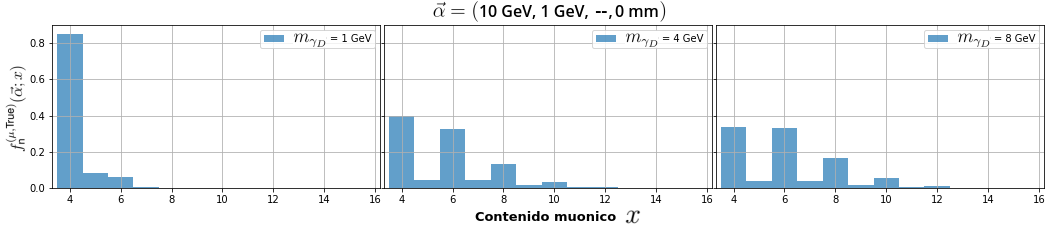
\includegraphics[width=1\textwidth]{Simulacion/imagenes/True_Entries.png}
\caption{Variación del contenido muónico de los eventos antes de pasar por el detector.}
\label{contenido_muonico}
\end{figure}

\begin{table}[!h]
\centering
\begin{tabular}{|cccccc|}
\hline
$m_{n_1} \textsf{(GeV)}$ & 
$m_{n_D} \textsf{(GeV)}$ & 
$m_{\gamma_D} \textsf{(GeV)}$ & 
$\tau c_{\gamma_D} \textsf{(mm)}$ & 
$\textsf{100} \cdot \Delta f^{(\geqslant 4\mu, \textsf{True})}_\textsf{rel}$ &
$\textsf{100} \cdot \Delta f^{(\geqslant 4\mu, \textsf{True})}_\textsf{n}$ \\
\hline
10 & 1 & 1 & 0 & 15.32 & 5.83 \\
10 & 1 & 4 & 0 & 60.43 & 43.18\\
10 & 1 & 8 & 0 & 66.16 & 51.70\\
\hline
\end{tabular}%}
\caption{Cambio del contenido muónico de procesos con variación de la masa de fotón oscuro $m_{\gamma_D}$ .}
\label{generacion0}
\end{table}

\subsubsection{Variación del momento transversal de los muones}

Analizar la señal \textbf{Dark}-\SUSY ~ mediante las propiedades de los muones sin la reconstrucción del detector dará una base de comparación y un mayor entendimiento de la teoría. Además, separar la información según los muones que provienen del decaimiento $h \rightarrow 2n_1 \rightarrow 2n_D + 2\gamma_D \rightarrow 2n_D + 4\mu$ del resto de los procesos se hace necesario para estudiar la reconstrucción conjunta de las señales. Se introduce la notación de las propiedades de una partícula $p= n_1, ~n_D, ~\gamma_D, ~\mu$, siendo la distribución de frecuencia dada por:
\begin{equation}
\textsf{W}^{(k/u)}_{p} (\textsf{X})
\end{equation}
 donde $\textsf{X}=\{m, \textsf{PT},\phi, \eta, \tau c , \textsf{T}, \textsf{D}_\textsf{0}, \textsf{D}_\textsf{Z}\}$ hace referencia a las propiedades a tratar, $k=\{\textsf{CMS}, \textsf{HL}, \textsf{True}\}$ hace referencia al detector usado y $u=\{\textsf{MSSMD, another},\textsf{ALL}\}$ declara si el origen de los datos es correspondiente a la teoría \textbf{Dark-}\SUSY ~ o no. 

\begin{figure}[!ht]
\centering
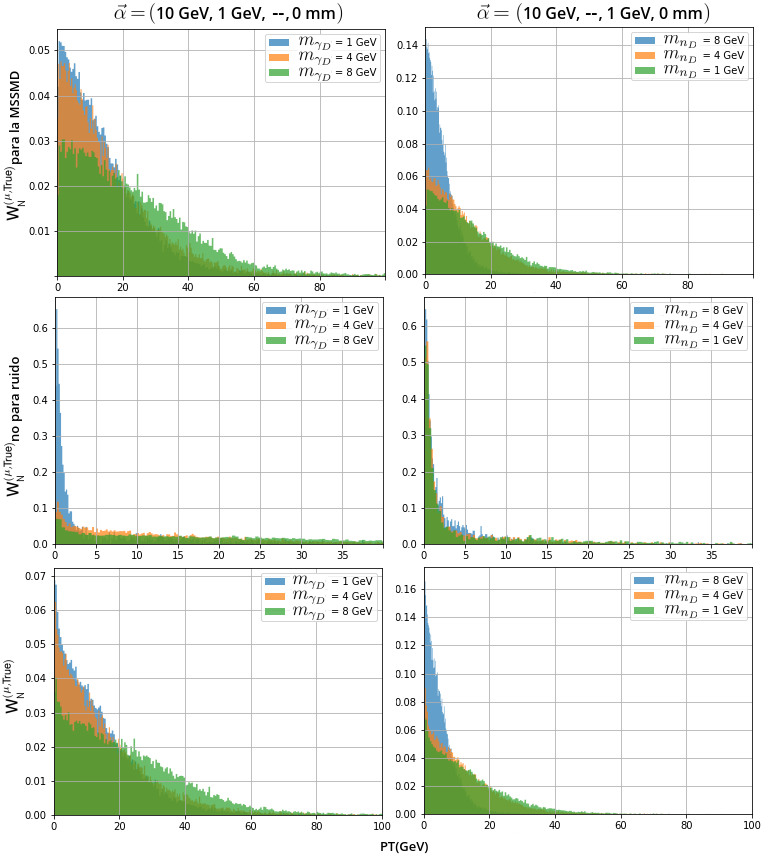
\includegraphics[width=.9\textwidth]{Simulacion/imagenes/True_PT4.png}
\caption{Variación de las distribuciones de los momentos transversales de los muones .}
\label{PT_mu_True}
\end{figure}

La distribución correspondiente al momento transversal de los muones $\textsf{W}^{(\textsf{True}/u)}_\mu (\textsf{PT})$ proveniente del decaimiento  \textbf{Dark-}\SUSY ~ ($u$ $=$ $\textsf{MSSMD}$)%$\textsf{PT}^{(\mu,\textsf{True})}_{(\textsf{MSSMD})}$
, de otros procesos secundarios ($u$ $=$ $\textsf{another}$) %$\textsf{PT}^{(\mu,\textsf{True})}_{(\textsf{notMSSMD})}$ 
y la unificación de los datos ($u$ $=$ $\textsf{ALL}$) %$\textsf{PT}^{(\mu,\textsf{True})}_{(\textsf{MSSMD+notMSSMD})} \equiv \textsf{PT}^{(\mu,\textsf{True})}$
se pueden visualizar en la Fig. \ref{PT_mu_True}. Con la comparación de las distribuciones se pudo evidenciar la variación de su morfología con el cambio del parámetro de generación masa del fotón oscuro $m_{\gamma_D}$ y del neutralino oscuro $m_{n_D}$. 


Las distribuciones muestran que el $\sim 95$\% de los muones correspondientes al decaimiento \textbf{Dark-}\SUSY ~ muestran su dominio para valores $\textsf{PT} < \textsf{80 GeV}$, para los muones resultantes de procesos de ruido tenemos $\textsf{PT} < \textsf{10 GeV}$. Además, se confirma una relación directa entre los estadísticos medios del momento transversal de los muones con el parámetro de generación masa del fotón oscuro $m_{\gamma_D}$, de forma inversa con el parámetro de masa del neutralino oscuro $m_{n_D}$.


\subsubsection{Características del fotón oscuro}
Se hace necesario estudiar las propiedades del fotón oscuro de nuestra señal sin detector para poder entender y caracterizar 

$\textsf{W}^{(\textsf{True/MSSMD})}_{\gamma}$

$\textsf{PT (GeV)}$

$\textsf{m (GeV)}$

$\textsf{T (mm)}$

$\textsf{D}_0 \textsf{(mm)}$

$\textsf{D}_\textsf{Z} \textsf{(mm)}$


\begin{figure}[!ht]
\centering
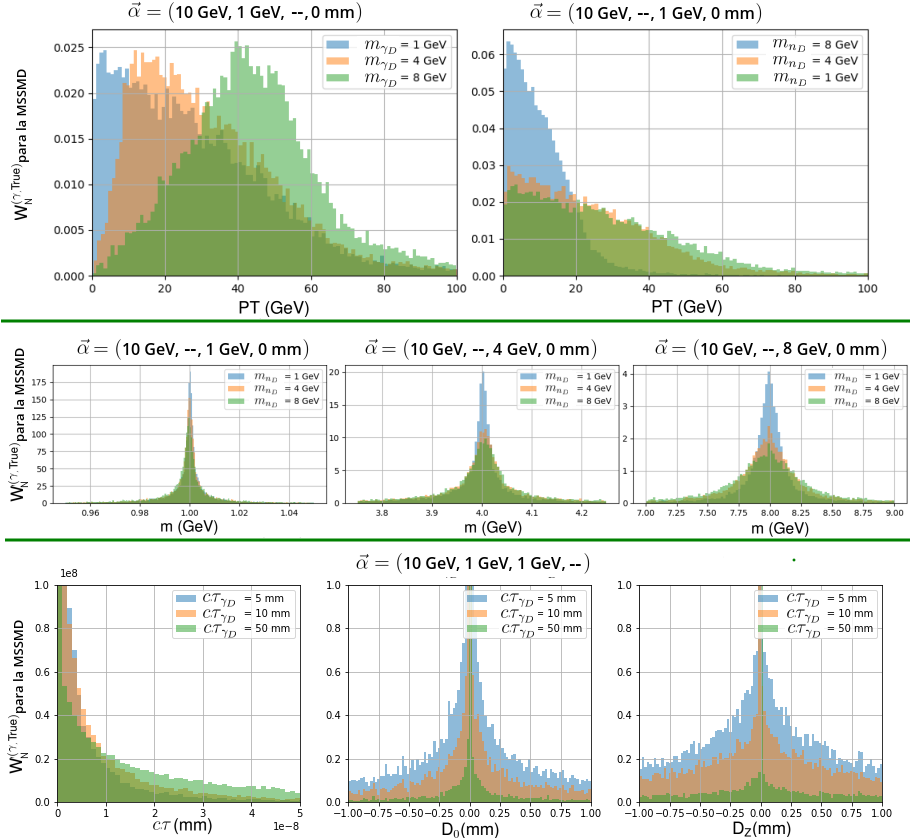
\includegraphics[width=.9\textwidth]{Simulacion/imagenes/True_PT5.png}
\caption{Variación de las propiedades del fotón oscuro con la variación de los parámetros de generación $m_{\gamma_D}$, $m_{n_D}$ y $\tau c_{\gamma_D}$.}
\label{PT_mu_True2}
\end{figure}









